\documentclass[11pt]{jarticle}

\usepackage{amsmath}
\usepackage[dvipdfmx]{graphicx}
\usepackage{hyperref}

\setlength{\oddsidemargin}{-0.7cm}
\setlength{\topmargin}{-1.5cm}
\setlength{\textwidth}{16.5cm}
\setlength{\textheight}{26cm}
\pagestyle{empty}

\begin{document}

\noindent
{\bf\large 「計算機実験II」実習課題 (2021/10/08更新)}
\\[-0.5em]

{\bf [モンテカルロ法]}
\begin{enumerate}

\item $X$と$Y$を$(0,1)$で一様分布するそれぞれ独立な(実数)確率変数とする。このとき$X^2$, $-\log X$, $XY$のそれぞれの確率密度関数と期待値を(解析的に)求めよ。また、実際に乱数を生成させてヒストグラムと期待値を計算し、解析的な結果と比較せよ。また、棄却法により、確率密度関数
  \begin{equation}
    P(x) = \begin{cases} 4x & 0 < x < 1/2 \\
      4(1-x) & 1/2 < x < 1 \\
      0 & \text{otherwise}
    \end{cases}
    \label{eqn:triangle}
  \end{equation}
  にしたがう一様乱数を生成せよ。ヒストグラムを作り、結果を確認せよ。さらに、確率密度関数(\ref{eqn:triangle})にしたがう$m=10$個の独立な確率変数の平均$Y=(1/m) \sum_{i=1}^m X_i$のヒストグラムを調べよ。$m$を増やしていくと分布はどのような形に近づくか予測し比較せよ。
  
\item 平均値$\mu_i$と共分散行列$\Sigma_{ij}$をもつ多次元正規分布にしたがう乱数の生成方法を考え実装し、平均値と共分散が正しく得られるかどうか確認せよ

\item 板状の物質による中性子の吸収/透過/反射をモンテカルロ法により計算するプログラムを作成せよ。吸収率$p_{\rm c}$、平均自由行程$\lambda^{-1}$を適当な値に仮定した上で、板の厚さ$D$を増やしたときに、吸収率・透過率・反射率がどのように変化するか調べよ。エラーバー(統計誤差)についても評価すること

\item 二次元正方格子上のランダムウォーク
  
\item マルコフ連鎖モンテカルロ法により、二次元正方格子イジング模型のエネルギーと比熱、磁化の二乗の期待値を計算せよ。システムサイズを$L=4, 6,8\cdots$と増やすと、これらの物理量の振る舞いがどのように変化するか調べよ。また、有限系のシミュレーション結果から、熱力学的極限における二次相転移の臨界温度と臨界指数を求める方法について調べよ

% \item 一次元イジング模型の物理量は、転送行列法を用いて厳密に計算可能である。マルコフ連鎖モンテカルロ法により計算した物理量と厳密解を比較し、一致するかどうか確認してみよ。システムサイズ依存性はどのようになっているか調べよ

% \item サイト数$N$の格子上の強磁性イジング模型を考える(二次元正方格子あるいは一次元鎖)。$N$個のスピンの状態を$N$ビットの整数で表すことにする($i$番目($i=0,\cdots,N-1$)の格子点のスピンの状態を$i$ビット目に保存)。この整数が表す状態のエネルギーおよび磁化を計算するプログラムを作成せよ。さらに、全ての状態についてボルツマン重みの和を取ることにより、自由エネルギーを計算せよ。低温でも桁あふれが起こらないよう注意すること。十分低温における自由エネルギーの値が基底状態エネルギー(全てのスピンが同じ方向に揃った状態)と一致することを確認せよ。有限温度のエネルギーと比熱の期待値を計算しプロットせよ。(可能であれば、結果がマルコフ連鎖モンテカルロ法と一致することを確認せよ)

\item 転送行列法は、一次元イジング模型の厳密解を求める方法として統計力学の教科書に載っているが、二次元以上のイジング模型の数値計算にも有用である(講義資料{\tt lecture-2-2.pdf} pp.24-29)。例えば、$L\times M$の二次元正方格子の場合、長さ$2^M$のベクトルを準備する必要があるが、$O(LM(2^M)^2)$の計算量で分配関数の計算を行うことができる。あるいは、幅$M$で長さ$L=\infty$の分配関数を$O(M(2^M))$で計算できる。必要メモリ量も計算量も$M$に関して指数関数的に増加するが、計算量は厳密な数え上げ($O(2^{LM})$)と比較すると非常に少ない(例えば$L=M=10$では、$2^{LM}=2^{100}\approx 10^{30}$に対して、$LM(2^M)^2=100 \times (2^{10})^2 \approx 10^{2+3\times2} = 10^{8}$)。$L=M$の場合には$M=10$以上、$L=\infty$の場合には$M=20$以上の計算を行うことができる。転送行列法のプログラムを作成し、二次元イジング模型の自由エネルギーを計算せよ。さらに、数値微分を用いて、エネルギー・比熱の温度依存性を計算せよ。(可能であれば、結果がマルコフ連鎖モンテカルロ法と一致することを確認せよ)

\item 二次元正方格子上の古典ハイゼンベルグ模型のマルコフ連鎖モンテカルロ法のプログラムを作成せよ。まず、三次元単位球面上に一様に分布するランダムベクトルの生成方法について考えよ。次にメトロポリス法のプログラムを作成し、エネルギー・比熱・磁化の二乗の期待値を計算、その温度依存性・サイズ依存性をプロットせよ。(可能であれば、二次元正方格子上のイジング模型に対するモンテカルロ計算の結果との比較を行い、定性的な違いについて議論せよ)

% \hspace*{-2em} {\bf [偏微分方程式]}

%% \item FTCS法を用いて一次元拡散方程式を適当な初期条件に対して解け。パラメータ$r=D\Delta t / \Delta x$を変化させて階の安定性・不安定性を確認せよ。FTCS法は、$(N+1) \times (N+1)$行列$A$を用いて${\bf u}^{n+1} = A {\bf u}^n$の形で表すことができる。数値対角化を用いて行列$A$の固有値を計算し、$r$の値によって固有値の分布がどのように変化するかを調べ、安定性について議論せよ。(可能であれば、陰解法の場合について同様の解析を行え)

%% \item 二次元波動方程式をFTCS法で解くプログラムを作成せよ。固定端条件と自由端条件の二通りの境界条件を設定し、境界での波の反射の様子を観察せよ。また、二次元空間中に波の速度(あるいは屈折率)の異なる2つの領域を作り、その境界で波の反射や屈折が起こることを確認せよ。(可能であればヤングの二重スリットの実験を再現してみよ)

%% \item 一次元一粒子の時間依存シュレディンガー方程式をFTCS法とクランク・ニコルソン法を用いて解く。初期状態として波束の波動関数$\Psi(x) \sim \exp [-(x-x_0)^2/(4\sigma^2) + i p_0(x-x_0)]$を考える。ポテンシャルがない場合($V=0$)に空間中を波束が伝搬していく様子を確認し、波動関数のノルム、位置・運動量・エネルギーの期待値の時間依存性を観察せよ。次に、中央にある高さのポテンシャル障壁を作り、壁の高さによって、透過率・反射率がどのように変化するかを調べよ
  
% \hspace*{-2em} {\bf [対角化]}

%% \item 一次元横磁場イジング模型
%%   \[
%%   H = - J\sum_{i=1}^N \sigma_i^z \sigma_j^z - \Gamma \sum_i \sigma_i^x
%%   \]
%%   の量子相転移を考える。$\sigma_i^z$を対角化する基底を考え、境界条件は周期境界条件とする。$N=3$の場合のハミルトニアンを$8\times8$行列の形で書き下せ。$N=3,4,5,\cdots$について、基底状態エネルギーと第一励起エネルギーを$\Gamma$の関数として計算し、$\Gamma/J < 1$では$N \rightarrow \infty$で基底状態は2重縮退、$\Gamma/J > 1$では1重縮退となることを示せ。また、磁化の二乗の期待値
%%   \[
%%   m^2 = \langle \Big( \frac{1}{N} \sum_i \sigma_i^z \Big)^2 \rangle
%%   \]
%%   を計算し、$\Gamma/J < 1$では有限の値、$\Gamma/J > 1$では零となることを確認せよ

%% \item ランダムに相互作用する古典スピン模型
%%   \[
%%   H = -J \sum_{i<j} \epsilon_{ij} \sigma_i^z \sigma_j^z
%%   \]
%%   ($\epsilon_{ij}$は正あるいは負)の基底状態の配位とそのエネルギーを求める。スピン数$N$は4から10程度を考える。まず、全探査により基底状態を求めよ。次に、量子アニーリング(lecture-2-4.pdf, p.11)でアニーリング時間$T$を変化させた時、正しい基底状態が得られる確率がどのように変化するか調べよ。

%% \item 3量子ビット加算器を講義資料(lecture-2-4.pdf, p.15)を参考に作成し、$2^3 \times 2^3$通りの入力に対して、正しい結果が得られることを確認せよ。さらに、状態の線形結合を入力とした場合に加算結果の線形結合が出力されることを確認せよ

% \hspace*{-2em} {\bf [常微分方程式]}

%% 以下の課題においては、必ず何種類かの時間刻み幅で実行し、収束の度合いを確認すること。また、2種類以上の積分法(例えば次数の異なるもの)で結果の妥当性を確認することが望ましい

%% \item 重力相互作用する$N$質点系の運動方程式
%%   \[
%%   m_i \frac{d^2 \mathbf{r}_i}{dt^2} = - \sum_{j \ne i} G m_i m_j \frac{\mathbf{r}_i - \mathbf{r}_j}{|\mathbf{r}_i - \mathbf{r}_j|^3} \qquad i = 1,\ldots,N
%%   \]
%%   は、$N \ge 3$の場合には求積可能ではないが、これまで様々な特殊解が得られている。3体問題($N=3$)においては、オイラーの直線解、ラグランジュの三角解に加え、3体が単一の閉曲線上を運動する「8の字解」が知られている。3体は等しい質量$m_i=1$を持ち、$z=0$の平面上を運動しているとする。また、重力定数$G=1$とする。初期条件として$(x_1,y_1)=(0,0)$, $(x_2,y_2)=-(x_3,y_3)$, $(\dot{x}_1,\dot{y}_1)=(0.695804,1.67860)$, $(\dot{x}_2,\dot{y}_2)=(\dot{x}_3,\dot{y}_3)=-\frac{1}{2}(\dot{x}_1,\dot{y}_1)$とする(重心と全運動量はゼロ)。初期条件$(x_2,y_2)$を変えて、シンプレクティック積分法により軌道を求め、「8の字解」となる条件を探せ。またその時の周期を見積もってみよ
%%   \begin{center}
%%     \resizebox{.4\textwidth}{!}{\includegraphics{figure-8.pdf}}
%%   \end{center}
  
%% \item 蔵本模型は同期現象を記述する数学モデルである。蔵本模型では、それぞれ異なる固有振動数$\omega_i$を持つ$N$個の振動子の間に非線形相互作用が働いている。支配方程式は以下の形で表される
%%   \[
%%   \frac{d\theta_i}{dt} = \omega_i + \frac{K}{N} \sum_{j=1}^N \sin(\theta_j - \theta_i) \qquad i=1,2,\ldots,N
%%   \]
%%   ここで、$\theta_i$は$i$番目の振動子の位相、$K$は結合定数である。結合定数$K$が小さいとき、振動子はインコヒーレントに振動するが、$K$がある臨界値$K^*$を超えると同期して振動するようになる。同期の度合いは複素秩序変数
%%   \[
%%   r(t) e^{i\Psi(t)} = \frac{1}{N} \sum_j e^{i\theta_j(t)}
%%   \]
%%   の絶対値$r(t)$により測ることができる。固有振動数$\omega_i$は平均0、分散1の正規分布に従いランダムに分布、また$t=0$において$\theta_i$は$[0,2\pi]$に一様分布しているとして、常微分方程式を数値的に解き、$r(t)$の時間依存性をプロットせよ。$N=64,128,256,\cdots$について、$r(t)$の長時間平均値の結合定数$K$の依存性を観察し、臨界点$K^*$を見積もってみよ。(高速化のヒント: 複素秩序変数$(r(t),\Psi(t))$を用いると、支配方程式の相互作用項は$K r \sin(\Psi-\theta_i)$と変形できる)

%% \item ローレンツ方程式は、カオス的な振る舞いを示す非線形方程式の代表例である
%%   \begin{align*}
%%     \dot{x} &= -\sigma x + \sigma y \\
%%     \dot{y} &= -xz + rx - y \\
%%     \dot{z} &= xy - bz
%%   \end{align*}
%%   パラメータを$\sigma=10$, $b=8/3$, $r=28$、初期条件を$(x,y,z)=(0,1,0)$として、Runge-Kutta法を用いてローレンツ方程式を数値的に解き、軌道を3次元プロットせよ。また、わずかにずらした初期値(例: $y=1 \rightarrow 1+\epsilon$)を考え、もとの軌道からのずれがどのように拡大していくかプロットせよ

%% \item 重力相互作用する$N$粒子系を考える
%%   \[
%%   V = - \sum_{j<k}^N \frac{Gm^2}{(r_{jk}^2 + \delta^2)^{1/2}} \qquad \text{($\delta$はエネルギーの発散を防ぐための小さな定数)}
%%   \]
%%   $t=0$で粒子は半径$R$の球内に一様にランダムに分布しているとする(棄却法で生成)。また、速度は分散$\sigma^2$のマクスウェルボルツマン分布($3N$次元正規分布)に従ってランダムに分布しているとする(それぞれの成分をBox-Muller法で生成)。運動エネルギーの初期値がポテンシャルエネルギーの絶対値に比べ十分に小さい時、この粒子系は自己重力で崩壊する。分散$\sigma^2$を調整して、ビリアル比$r_\text{v} \equiv K/|V|$が0.1, 0.2, 0.3, 0.4となるような初期速度分布を準備し、シンプレクティック積分法により、ポテンシャルエネルギー、運動エネルギー、ビリアル比、中心にできるコアの半径の時間依存性をプロットせよ。$G=R=M(\equiv Nm)=1$となる単位系を使い、ソフトニングパラメータ$\delta=0.01$、粒子数$N$は$10^3$程度で$t=10$程度まで計算してみよ

%% \item アルゴン原子間の相互作用はレナード・ジョーンズ型ポテンシャル
%%   \[
%%   V = - \sum_{j<k}^N \epsilon \Big[\Big(\frac{\sigma}{r_{jk}}\Big)^{12} - 2 \Big(\frac{\sigma}{r_{jk}}\Big)^6\Big] \qquad \text{($\epsilon / k_B = 119.8$ K, $\sigma = 3.822$ \AA)}
%%   \]
%%   でよく記述される。1片の長さ$L$の箱の中に$N$個のアルゴン原子が入っている状況を考える。周期境界条件を考え、ポテンシャルエネルギーはminimum image conventionにより計算する。シンプレクティック積分法により、温度、圧力、内部エネルギーの平均値を計算するプログラムを作成せよ。$m=\sigma=\epsilon=1$となる単位系を使い、時間きざみ幅は0.005程度に取る。粒子の初期位置は面心立方格子とする。まず、$N=32$の系について計算を行い、速度を反転した場合に初期状態に戻ることを確認せよ。次に$N=108$、数密度$\rho=N/V=1.2$の系について、$t=10$まで10ステップごとに温度$T=1$となるように速度スケーリング、その後$t=30$までエネルギー一定のシミュレーションを行い、温度、圧力、1粒子あたりの内部エネルギーの期待値を計算せよ

%% \item Nose-Hoover Chain法を用いた分子動力学法により、調和ポテンシャルあるいは非調和ポテンシャル中の1粒子のカノニカル分布を調べる
%%   \begin{align*}
%%     \frac{dx}{dt} &= \frac{p}{m} \\
%%     \frac{dp}{dt} &= -\frac{\partial V}{\partial x} - \frac{p_s}{Q} p \\
%%     \frac{dp_s}{dt} &= \frac{p^2}{m} - k_B T - \frac{p_r}{Q} p_s \\
%%     \frac{dp_r}{dt} &= \frac{p_s^2}{Q} - k_B T
%%   \end{align*}
%%   $m=1$, $Q=1$, $k_BT=1$として、4次のRunge-Kutta法で運動方程式を解き、その位相空間上での軌道を確認せよ(時間刻み$\Delta=0.01$で$t=10^4$程度まで計算せよ)。また、座標$x$と運動量$p$のヒストグラムを作成し、カノニカル分布となっていることを確認せよ。一方、自由度1のNose-Hoover熱浴(上の式で$p_r$のないもの)の場合には、熱平衡状態とはならないことを示せ

% \clearpage
  
% \hspace*{-2em} {\bf [最適化]}

%% \item Rosenbrock関数
%%   \begin{align*}
%%     f(x,y) = (a - x)^2 + b(y-x^2)^2 \qquad (a=1, b=5)
%%   \end{align*}
%%   は、細長い曲がった谷の中に最小点$(x,y)=(a,a^2)$をもつ。Gnuplotにより等高線を描き、全体の形を確認せよ。次に、最急降下法、勾配降下法、共役勾配法により最小点を求めるプログラムを作成し、収束の様子($xy$平面上での軌跡や真の最小点からの距離のステップ数依存性)を調べよ。初期位置は$(x,y)=(-1,-1)$とする

%% \item 共役勾配法を用いて、Dirichlet型の境界条件のもとでの二次元Poisson方程式(あるいはLaplace方程式)の解を求めるプログラムを作成せよ。実行時間のメッシュ数依存性をLU分解を用いた場合と比較せよ(参考: 計算機実験I 講義資料{\tt lecture-1-5.pdf} p.5)。Poisson方程式を行列形式に書き直すことが難しい場合には、{\tt poisson.h}を参考にしてもよい(行列生成{\tt poisson\_dense.c}、行列ベクトル積{\tt poisson\_sparse.c}、LU分解による求解{\tt poisson\_lu.c}のテストプログラムもあり)

%% \item 測定データ{\tt measurement3.dat}を関数$y=f(x)=ax+be^{−(x−c)^2}$で最小二乗フィッティングしよう。パラメータ$a, b, c$を、勾配降下法、Nelder-Mead法などを用いて残差を最小化することにより推定せよ
%%   \begin{center}
%%     \resizebox{.4\textwidth}{!}{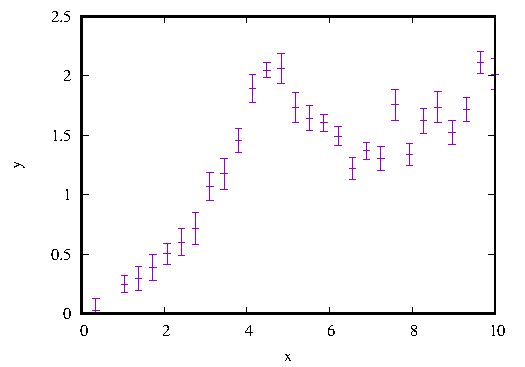
\includegraphics{optimization/measurement3.pdf}}
%%   \end{center}
  
%% \item Nelder-Meadの滑降シンプレクティック法を用いて、課題21のRosenbrock関数の最小点を探索するプログラムを作成せよ

%% \item $d$次元Rastrigin関数
%%   \begin{align*}
%%     f(x) = Ad+\sum_{i=1}^d [x_i^2 - A \cos (2 \pi x_i)] \qquad (A=10, -5.12 \le x_{i} \le 5.12)
%%   \end{align*}
%%   は$x=0$に最小点をもつが、それ以外に多数の極小点が存在する。Gnuplotにより$d=2$の場合の等高線を描き、極小の位置を確認せよ。次に、シミュレーテッドアニーリングにより、Rastrigin関数の最小点を探索するプログラムを作成せよ。「温度」$T$は、アニーリング時間$\tau$をかけて
%%   \[
%%   T(t) = T_0 (1 - t/\tau)
%%   \]
%%   のように線形に減少させるとする。初期温度$T_0$はRastrigin関数の最大値よりも十分大きくとる。$d=3$の場合について、最小点$x=0$を見出す確率の$\tau$依存性を調べよ

%% \item $n \times n$マス目に$1\sim n^2$の自然数を並べた魔法陣をシミュレーテッドアニーリングにより生成しよう。正しい魔法陣では、行・列・対角線の和はすべて$M = n(n^2+1)/2$とならなければならない。状態(=数字の並べ方) $C$に対して、エネルギーを
%%   \[
%%   E(C) = \sum_{\rm row} (S_r-M)^2 + \sum_{\rm col} (S_c-M)^2 + \sum_{\rm diag} (S_d-M)^2
%%   \]
%%   (ただし、$S_r, S_c, S_d$はそれぞれ、$r$行目、$c$列目、2方向の対角線の数字の和)と定義すると、「基底状態」$E(C)=0$は正しい魔法陣(の一つ)を与える。モンテカルロによる状態更新は、まず$1\sim n^2-1$の自然数$i$をランダムに選び、数字$i$と$i+1$の位置を入れ替える操作を考えればよい。$n=3,4,5,6$の場合について、正しい魔法陣を見出す確率のアニーリング時間依存性を調べよ。また、最急下降法の結果との比較も行え
  
% \hspace*{-2em} {\bf [その他]}

% \item 「\href{https://github.com/utphys-comp/handbook/releases/download/handbook-2019/handbook.pdf}{計算機実験ハンドブック}」の1.3節にEmacs以外のエディタの説明(vi (vim)、nano)を追加

% \item 「\href{https://github.com/utphys-comp/handbook/releases/download/handbook-2019/handbook.pdf}{計算機実験ハンドブック}」の第2章「C言語入門」のC++言語版を追加

\end{enumerate}  

%% \renewcommand{\thefootnote}{\fnsymbol{footnote}}
%% \footnote[0]{Gnuplotでアニメーションを作成する方法については、 \url{https://slpr.sakura.ne.jp/qp/gnuplot-animation/} に様々な例が示されている}
  
\noindent
課題は順次追加予定 \\[-0.5em]

\end{document}
